% Chapter 2

\chapter{Methods} % Main chapter title

\label{ChapterX} % For referencing the chapter elsewhere, use \ref{Chapter2} 

% \lhead{Chapter 2. \emph{Methods}} % This is for the header on each page - perhaps a shortened title

%----------------------------------------------------------------------------------------

\section{Cell Cultures}
A9 ouab\textsuperscript{r}l1 cells, a derivative from the original HGPRT\textsuperscript{-} L-cell line A9 represent a clone resistant to 10\textsuperscript{-3} M ouabain after nitrosoguanidine mutagenesis \cite{pmid14213660}.
NB324K cells are a clone of SV40-transformed \nomenclature{SV40}{Simian vacuolating virus 40 or Simian virus 40} human newborn kidney cells \cite{pmid13911591}. The SV40 large T antigen was detected by immunofluorescent \nomenclature{IF}{Immunofluorescence microscopy} staining with monoclonal antibodies (mAb) \cite{pmid6169844}. \nomenclature{mAb}{Monoclonal antibody} However, NB324K cells do not produce infectious SV40 spontaneously.
Both cell lines, A9 mouse fibroblasts and NB324K cells, were routinely propagated under a minimal number of passages in Dulbecco's Modified Eagle Medium (DMEM) (see Table~\ref{Media}, p.~\pageref{Media}) supplemented with 5~\% of heat inactivated fetal calf serum (FCS) at 37~\textcelsius~in 5~\% CO\textsubscript{2} atmosphere.

\nomenclature{FCS}{Fetal calf serum} 
\nomenclature{DMEM}{Dulbecco modified Eagle's medium}

\subsection{Freezing and thawing of cells}
Before use, the A9 mouse fibroblasts or NB324K cells were thawed at 37 \textcelsius~ and cultured in 5 mL of pre-warmed DMEM (see Table~\ref{Media}, p.~\pageref{Media}) supplemented with 5~\% FCS. The medium was replaced every 3 to 4 days. 
In order to freeze the cells for long storage in liquid nitrogen they were passed the day before in DMEM containing 10~\% FCS, to ensure exponential growth. Subsequently, 7.5~\% DMSO was added and the cells were frozen slowly at -70 \textcelsius~ over night before transfer to liquid nitrogen.

%----------------------------------------------------------------------------------------

\section{Virus Stocks}
\label{Virus Stocks}
Stocks of MVM without detectable levels of VP3 were propagated on A9 mouse fibroblast monolayers. As soon as the cytopathic effect was complete, the supernatant (SN) was collected and pre-cleared from cell debris by low-speed centrifugation. Thereby, intracellular VP3 rich capsids were discarded. In order to remove low-molecular contaminants, virus containing SN was pelleted through 20~\% sucrose cushion in PBS by ultra-centrifugation. Virus titers were determined by quantitative PCR (qPCR) (see Section~\ref{qPCR}, p.\pageref{qPCR}) as DNA-packaged particles per microliter.   

\nomenclature{SN}{Supernatant}
\nomenclature{qPCR}{Quantitative PCR} 
\nomenclature{PCR}{Polymerase chain reaction}

\subsection{Separation of empty and full capsids}

Sucrose purified capsids were prepared as previously described in Section~\ref{Virus Stocks}, p.~\pageref{Virus Stocks}. The virus pellet was resuspended in 10 mL PBS. Caesium chloride was added to a density of 1.38 g/mL adjusted by refractometry ($\eta$=1.371) at 4~\textcelsius. The gradient was centrifuged to equilibrium for 24 h at \np{41000} rpm and 4~\textcelsius~in a Beckman SW-41 Ti rotor. Gradients were fractionated and tested for intact capsids by dot blot analysis using B7 mAb (see Table~\ref{Primary antibodies}, p.~\pageref{Primary antibodies}). CsCl was depleted from the corresponding fractions by size-exclusion chromatography through PD-10 desalting columns (GE Healthcare) and the capsids were concentrated in Amicon\textsuperscript{\textregistered} centrifugal filter devices (Merck Millipore) when required.          
   
   


\section{Freezing bacteria stocks in glycerol}
Bacteria were frozen in dry ice. A volume of 700 $\mu$L of the bacteria culture that was grown over night in LB-medium (see Table~\ref{Media}, p.~\pageref{Media}) was mixed with 300 $\mu$L of 50~\% glycerol in a cryotube. In order to mix well the glycerol the cryotube was vortexed intensively. Following snap-freeze in dry ice the bacteria were stored at -70 \textcelsius.


\section{Fast protein liquid chromatography (FPLC)}

\begin{figure}[H]
\centering
  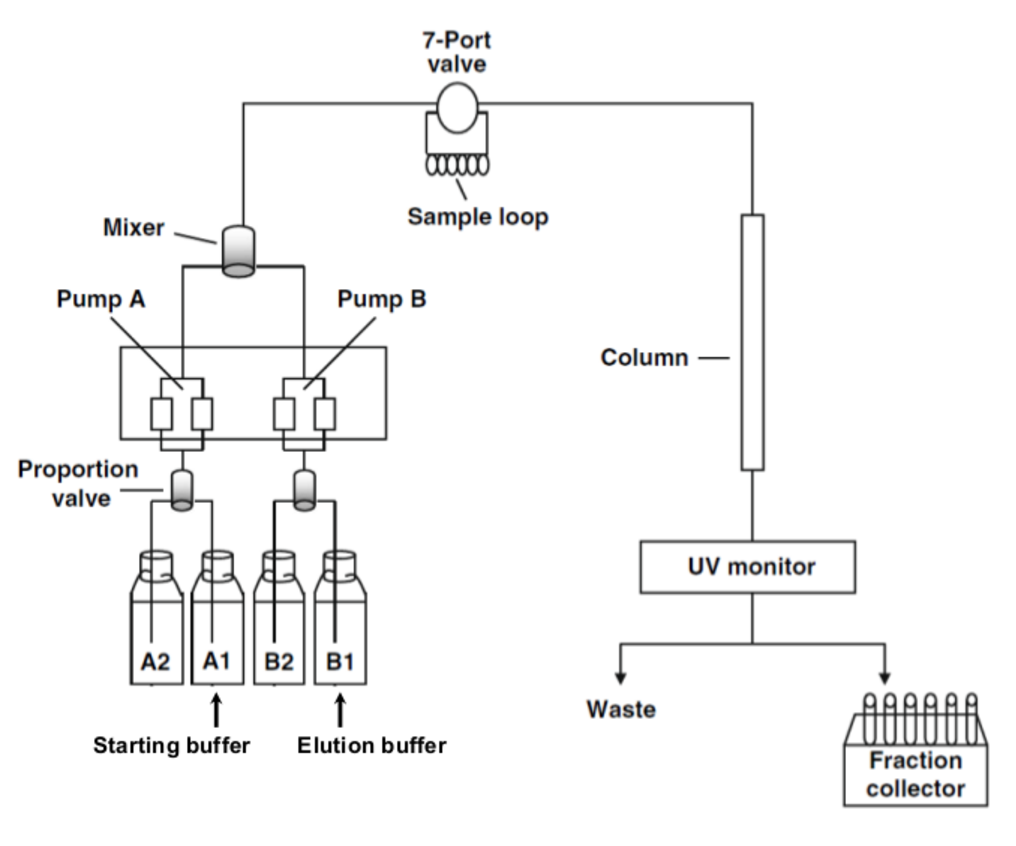
\includegraphics[scale=0.7]{FPLC}
  \caption[Schematic outline of the ÄKTA purifier FPLC chromatography system.]
   {Schematic outline of the ÄKTA purifier FPLC chromatography system. This figure was adapted from \cite{pmid20978981}.} 
\label{FPLC}
\end{figure}


\subsection{Anion-exchange chromatography (AEX)}
\label{AEX}
A Mono Q\textsuperscript{\texttrademark} HR 5/5 (Pharmacia) column (5 x 50 mm) was used to analyse virus samples. The Mono Q column was connected to the ÄKTA purifier 10 chromatography system (GE Healthcare) that was operated by the unicorn control software (GE Healthcare). The Mono Q\textsuperscript{\texttrademark} column was equilibrated with five column volumes (CV) starting buffer (see Table~\ref{AEX buffers}, p.~\pageref{AEX buffers}). Samples (1 mL) containing at least 10\textsuperscript{10} DNA-containing virus particles in sample buffer (see Table~\ref{AEX buffers}, p.~\pageref{AEX buffers}) were applied to the Mono Q\textsuperscript{\texttrademark} column trough a 2 mL injection loop. Following sample application the loop and the column were rinsed with six CV starting buffer. In order to elute the bound proteins, a linear salt gradient (0-2 M NaCl) was applied by gradually increasing the concentration of the elution buffer (see Table~\ref{AEX buffers}, p.~\pageref{AEX buffers}). The total elution volume of 24 CV was split into fractions of 185 $\mu$L which were collected in 96-well plates. The flow rate was constantly kept at 1.5 mL/min and the salt concentration was monitored by measuring the electrical conductivity. Viral genomes in each fraction were quantified by qPCR (see Section~\ref{qPCR}, p.~\pageref{qPCR}).  

Occasionally, the Mono Q\textsuperscript{\texttrademark} column needed to be washed. Increased back-pressure, color change at the top of the column, decreased sample recoveries, or loss of resolution indicate that the column matrix requires regeneration. In order to circumvent such problems, the column was washed every tenth run. To eluate contaminants that tightly stick to the column the following harsh conditions were applied to the reversed (bottom to top) Mono Q\textsuperscript{\texttrademark} column. 500 $\mu$L 2 M NaCl solution was injected and subsequently, the column was rinsed with water. Then, 500 $\mu$L 2 M NaOH solution was injected and the column was rinsed with water. Finally, 500 $\mu$L 75~\% acetic acid was injected before the column was re-equilibrated with starting buffer (see Table~\ref{AEX buffers}, p.~\pageref{AEX buffers}).             

All buffers were filtered and degassed before application to the Mono Q\textsuperscript{\texttrademark} column.

\nomenclature{CV}{Column volume}


\subsection{Chromatofocusing (CF)}
\label{CF}

A Mono P\textsuperscript{\texttrademark} 5/200 GL (GE Healthcare) column (5 x 200 mm) was used to determine the isoelectric points (pI) of virus samples.  The column was connected to the ÄKTA purifier 10 chromatography system (GE Healthcare) that was operated by the unicorn control software (GE Healthcare). The Mono P\textsuperscript{\texttrademark} column was equilibrated with two CV of buffer A (see Table~\ref{CF buffers}, p.~\pageref{CF buffers}). Samples (500 uL) containing 10\textsuperscript{10} DNA-containing virus particles in buffer A (see Table~\ref{CF buffers}, p.~\pageref{CF buffers}) were applied to the Mono P\textsuperscript{\texttrademark} column through a 1 mL injection loop. Following sample application, the loop and the column were rinsed with 10 mL buffer A (see Table~\ref{CF buffers}, p.~\pageref{CF buffers}). Bound viruses were eluted by applying buffer B (see Table~\ref{CF buffers}, p.~\pageref{CF buffers}) to the column. Buffer B contains the acidic ampholyte solution, thus gradually lowering the pH within the column. The total elution volume of 7 CV was split into fractions of 250 $\mu$L which were collected in 96-well plates. The flow rate was constantly kept at 0.5 mL/min and the pH was monitored. Viral genomes in each fraction were quantified by qPCR (see Section~\ref{qPCR}, p.~\pageref{qPCR}).      

All buffers were filtered and degassed before application to the Mono P\textsuperscript{\texttrademark} column.

\nomenclature{pI}{Isoelectric point}

\section{Quantitative PCR (qPCR)}
\label{qPCR}
Amplification of MVM DNA and real-time detection of PCR products were performed by using CFX96 technology (BioRad) with iTaq\textsuperscript{\texttrademark} Universal SYBR\textsuperscript{\textregistered} Green Supermix (see Table~\ref{Kits}, p.~\pageref{Kits}). PCR was carried out by using the hot-start iTaq\textsuperscript{\texttrademark} DNA polymerase (BioRad) following the manufacturer’s guide-lines. Viral DNA was isolated using the DNeasy blood and tissue kit (see Table~\ref{Kits}, p.~\pageref{Kits}). Elution of the purified vDNA was carried out using 100 $\mu$L elution buffer. As templates 2 $\mu$L of the isolated viral DNA were used for the PCR reaction as outlined in Table~\ref{Master mix}.\\

\begin{table}[H]
\begin{center}
\begin{tabular}{l r r}
\textbf{Component} & \textbf{Amount} & \textbf{Final concentration}\\
\hline
dH\textsubscript{2}O, PCR grade & 6 $\mu$L & -\\
Forward primer (CR3), 10 pM & 1 $\mu$L & 0.5 pM\\
Reverse primer (CR4), 10 pM & 1 $\mu$L & 0.5 pM\\
2x IQ\textsuperscript{\texttrademark} SYBR\textsuperscript{\textregistered} Green Supermix & 10 $\mu$L & 1$\times$\\
\hline
\textbf{Total volume} & \textbf{18 $\boldsymbol{\mu}$L} & \\
\end{tabular}
\end{center}
\caption[Master mix for quantitative PCR]{Master mix for quantitative PCR. In order to minimize pipetting errors a master mix was prepared. Following preparation the master mix was distributed across the 96 well plates. The master mix contains all the ingredients which are required for the DNA amplification except the initial DNA template that differs among the samples.}
\label{Master mix}
\end{table} 

To ensure accurate quantification, the 96-well plates containing master mix and template DNA were shortly spun and transferred into the BioRad CFX96 unit. The PCR program used for quantification of viral DNA is depicted in Table~\ref{PCR conditions}.

\begin{table}[H]
\begin{center}
\begin{tabular}{r l r r}
\textbf{Cycles} & \textbf{Step} & \textbf{Temperature} & \textbf{Time}\\
\hline
\par\smallskip
1x & Initial denaturation & 95 \textcelsius & 300 s\\
40x & Denaturation & 95 \textcelsius & 15 s \\
 & Annealing & 61 \textcelsius & 15 s \\
\par\smallskip 
 & Extension & 72 \textcelsius & 15 s \\
1x & Final denaturation & 95 \textcelsius & 60 s \\
1x & Melting curve & 65 \textcelsius~up to 95 \textcelsius & 0.1 \textcelsius/s \\
\end{tabular} 
\end{center} 
\caption[PCR conditions]
   {PCR conditions for the amplification and real-time detection of MVM DNA.}
\label{PCR conditions}
\end{table}

To provide standards for sample quantification, serially diluted plasmids containing the entire MVM genomic DNA were used.
For cell number variations that may exist between the samples, the number of applied cells per PCR reaction needed to be quantified for normalization as well. For this purpose quantification of cellular $\beta$-actin gene was performed. After normalization, direct comparison of the results is possible. $\beta$-actin quantification was carried out with the same PCR conditions outlined in Table~\ref{PCR conditions}, p.~\pageref{PCR conditions} with the annealing temperature (60~\textcelsius) as the only exception.

In Table~\ref{Primers} all primers are listed which were used for MVM genome or $\beta$-actin gene quantification. 
\begin{table}[H]
\begin{center}
\begin{tabular}{l l}
\textbf{Primer} & \textbf{Sequence}\\
\hline
CR3 & 5'-GACGCACAGAAAGAGAGTAACCAA-3'\\
CR4 & 5'-CCAACCATCTGCTCCAGTAAACAT-3'\\
Mouse $\beta$-actin forward & 5'-TGGCACCACACCTTCTACAATGA-3' \\
Mouse $\beta$-actin reverse & 5'-CCGCTCGTTGCCAATAGTGA-3' \\
Human $\beta$-actin forward & 5'-TGCTGTCCCTGTATGCCTCTG-3' \\
Human $\beta$-actin reverse & 5'-AATGCCTGGGTACATGGTGGT-3' \\
\end{tabular} 
\end{center} 
\caption[Primers]{Different primers that were used for qPCR.}
\label{Primers}
\end{table}


\section{Virus infection} 

A9 or NB324K cells (10\textsuperscript{5} for qPCR or 3~$\times$~10\textsuperscript{6} for AEX) were infected with MVM (\np{5000} DNA-containing particles per cell, corresponding to approximately 10 PFU/cell) for 1 h at 4~\textcelsius~for binding. Unbound virus was removed by washings and incubated at 37~\textcelsius~to initiate infection. At progressive times post-internalization total cellular DNA was extracted for qPCR analysis (see Section~\ref{qPCR}, p.~\pageref{qPCR}) or cells were fractionated (see Section~\ref{Fractionation}, p.~\pageref{Fractionation}) and subjected to AEX (see Section~\ref{AEX}, p.~\pageref{AEX}).    



\section{Transfection}
NB324K cells at a confluence of 70 \% were trypsinized and resuspended in 10 mL of DMEM (see Table~\ref{Media}, p.~\pageref{Media}) supplemented with 10 \% FCS. A total amount of 10\textsuperscript{6} cells were used for transfection with the AMAXA\textsuperscript{\texttrademark} nucleofector\textsuperscript{\texttrademark}~\RM{2} device following the manufacturer’s instructions. Transfection was carried out with 5 $\mu$g of the infectious clone of MVM (see Section~\ref{IC}, p.~\pageref{IC}, \cite{pmid6345805}) using the V-001 program. As a transfection reagent, AMAXA\textsuperscript{\textregistered} Cell Line Nucleofector\textsuperscript{\textregistered} Kit V (see Table~\ref{Kits}, p.~\pageref{Kits}) was used. Following transfection the weakened cells were maintained in 1.5 mL of pre-warmed culture medium and after 6 h, the culture medium was replaced with an equal amount of pre-warmed culture medium. The cells were further incubated for the required times.
        

\section{Cell fractionation}
\label{Fractionation}
\subsection{Nuclei isolation}
Isolation of A9 and NB324K nuclei was performed by using the Nuclei EZ Prep Nuclei Isolation Kit (see Table~\ref{Kits}, p.~\pageref{Kits}) following the manufacturer’s instructions. In order to obtain highly pure nuclear fractions, the isolated nuclei were pelleted through a sucrose gradient by low speed centrifugation at 500 g for 10 min. Extracted nuclei were lysed in nuclei lysis buffer (see Table~\ref{General buffers}, p.~\pageref{General buffers}) at 4~\textcelsius~for 30 min. Following vortexing thoroughly the nuclear lysate was passed through a 27 G needle 10 times. Debris was removed by centrifugation at \np{10000} rpm for 10 min at 4~\textcelsius.      

\subsection{Extraction of the cytoplasm}
Cytoplasmic fractions were extracted in cell lysis buffer (see Table~\ref{General buffers}, p.~\pageref{General buffers}) at 4~\textcelsius~for 30 min. Following vortexing thoroughly, intact nuclei and cell debris was removed by centrifugation at \np{10000} rpm for 10 min at 4~\textcelsius. 




\section{Immunoprecipitation (IP)}
\textit{In vitro} treated viruses or viruses from cell extracts were transferred to LoBind tubes that were pre-blocked with PBS containing 1~\% bovine serum albumin (PBSA 1~\%). The volume was adjusted to 200 $\mu$L with PBSA 1~\%. The antibody was added in excess and incubated with the viral capsids for 1 h at 4 \textcelsius~ on a rotary shaker. Subsequently, 20 $\mu$L protein G-agarose beads were added. Following overnight incubation at 4 \textcelsius~ and centrifugation at \np{2500} rpm for 5 min the supernatant was discarded. The beads were washed 4 times with PBSA 1~\%. To remove the BSA an additional wash step was carried out with PBS. Finally, the beads were frozen at -20 \textcelsius~ until further use or immediately processed. 

\nomenclature{IP}{Immunoprecipitation}

\section{Dot Blot}
Viruses (10\textsuperscript{8} in 2 $\mu$L) were spotted on a nitrocellulose membrane. The membrane was blocked for 20 min with TBST containing 5~\% milk. The primary antibody was diluted in TBST supplemented with 1~\% milk and incubated for 30 min at room temperature. Unbound antibody was removed by washing the membrane 3 times for 5 min with TBST containing 1~\% milk. The HRP-coupled secondary antibody was diluted 1:\np{20000} in TBST supplemented with 1~\% milk and added to the membrane for 30 min. Excess secondary antibody was removed by the same procedure as aforementioned for the primary antibody. The membrane was developed by exposure to photo films.    


\section{SDS-PAGE and Western blotting (WB)}

Immunoprecipitated capsids were dissolved in 20 $\mu$L protein loading buffer (reference) containing 2~\% SDS and 10~\% glycerol. The samples were boiled at 96 \textcelsius~ for 8 min. Viral proteins were separated through a NuPAGE\textsuperscript{\textregistered} 10~\% Bis-Tris Gel (Invitrogen). The XCell Sure Lock\textsuperscript{\texttrademark} Electrophoresis Cell (Invitrogen) was used to separate the proteins. The gel was first run at 30 V for 10 min to stack the proteins. In this way, sharper bands could be achieved. Separation of the different proteins was accomplished at 200 V. Following separation, the proteins were blotted on a methanol activated, porous, 0.2 $\mu$m polyvinylidene fluoride (PVDF) Immobilon\textsuperscript{\textregistered} Transfer Membrane (EMD Millipore). Blotting was carried out at 30 V for 1 h 10 min using XCell II\textsuperscript{\texttrademark} Blot Module (Invitrogen). 
The membrane was blocked in TBS-T buffer (reference) supplemented with 5~\% milk overnight at 4 \textcelsius. Subsequently, the membrane was probed with a polyclonal rabbit antibody against linear MVM-VP epitopes that was diluted 1:\np{2000} in 3 mL TBS-T containing 1~\% milk. The first antibody (reference) was incubated for 1 h at RT. The PVDF membrane was washed in TBS-T for a total 90 min with many buffer replacements. Subsequently, the horseradish peroxidise conjugated secondary antibody (goat $\alpha$-rabbit-HRP, reference) was added for 1 h at RT. This secondary goat anti-rabbit antibody was diluted 1:\np{20000} in TBS-T supplemented with 1~\% milk. To deplete remaining antibodies, the membrane was washed in the same way as described above except for a final wash step with TBS (reference). VP1, VP2, and possibly VP3 were visualized by a chemiluminescence system (SuperSignal West Dura Extended Duration Substrate, reference) following the manufacturer’s instructions. Following this treatment, the PVDF membrane was exposed to a film (Amersham Hyperfilm\textsuperscript{\texttrademark} ECL, reference). Finally, the film was developed using Anatomix Developer Replenisher Solution and Fixer and Replenisher Solution (reference).

\section{Enzymatic reactions}
 
All enzymatic reactions were performed with 10\textsuperscript{8} virus particles in a reaction volume of 50 $\mu$L. Viruses were incubated in PBS for 1.5 h at 37~\textcelsius~with 0.5 mg/mL chymotrypsin (see Table~\ref{Enzymes}, p.~\pageref{Enzymes}). The reaction was blocked by adding 100 $\mu$M chymostatin (see Table~\ref{Chemicals}, p.~\pageref{Chemicals}). 

Phosphatase lambda treatment (\np{2000} Units, see Table~\ref{Enzymes}, p.~\pageref{Enzymes}) was performed in 50 mM Tris-HCl, 100 mM NaCl, 2 mM MnCl\textsubscript{2}, 5 mM DTT, pH 7.8 for 3 h at 37~\textcelsius~in PBSA 1 \% pre-blocked Protein LoBind eppendorf tubes. Phosphatase lambda was inactivated by supplementing the enzymatic reaction with 1 mM Na\textsubscript{3}VO\textsubscript{4} and 1 mM NaF. 

Free DNA was digested using 50 Units DNaseI (see Table~\ref{Enzymes}, p.~\pageref{Enzymes}) in 1$\times$ incubation buffer according to the manufacturer’s protocol. DNaseI was inhibited by incubation at 75~\textcelsius~for 15 min. 

Negative controls were incubated in the same buffers for the same time.




%----------------------------------------------------------------------------------------

